\documentclass{subfiles}

\begin{document}
    Zuerst kann man das verlauf des Potentials $V(x,y)$ zeichnen. Hier ist die reelen Werte für die Masse und Abstände eingetragen.
    \begin{figure}[H]
        \centering
        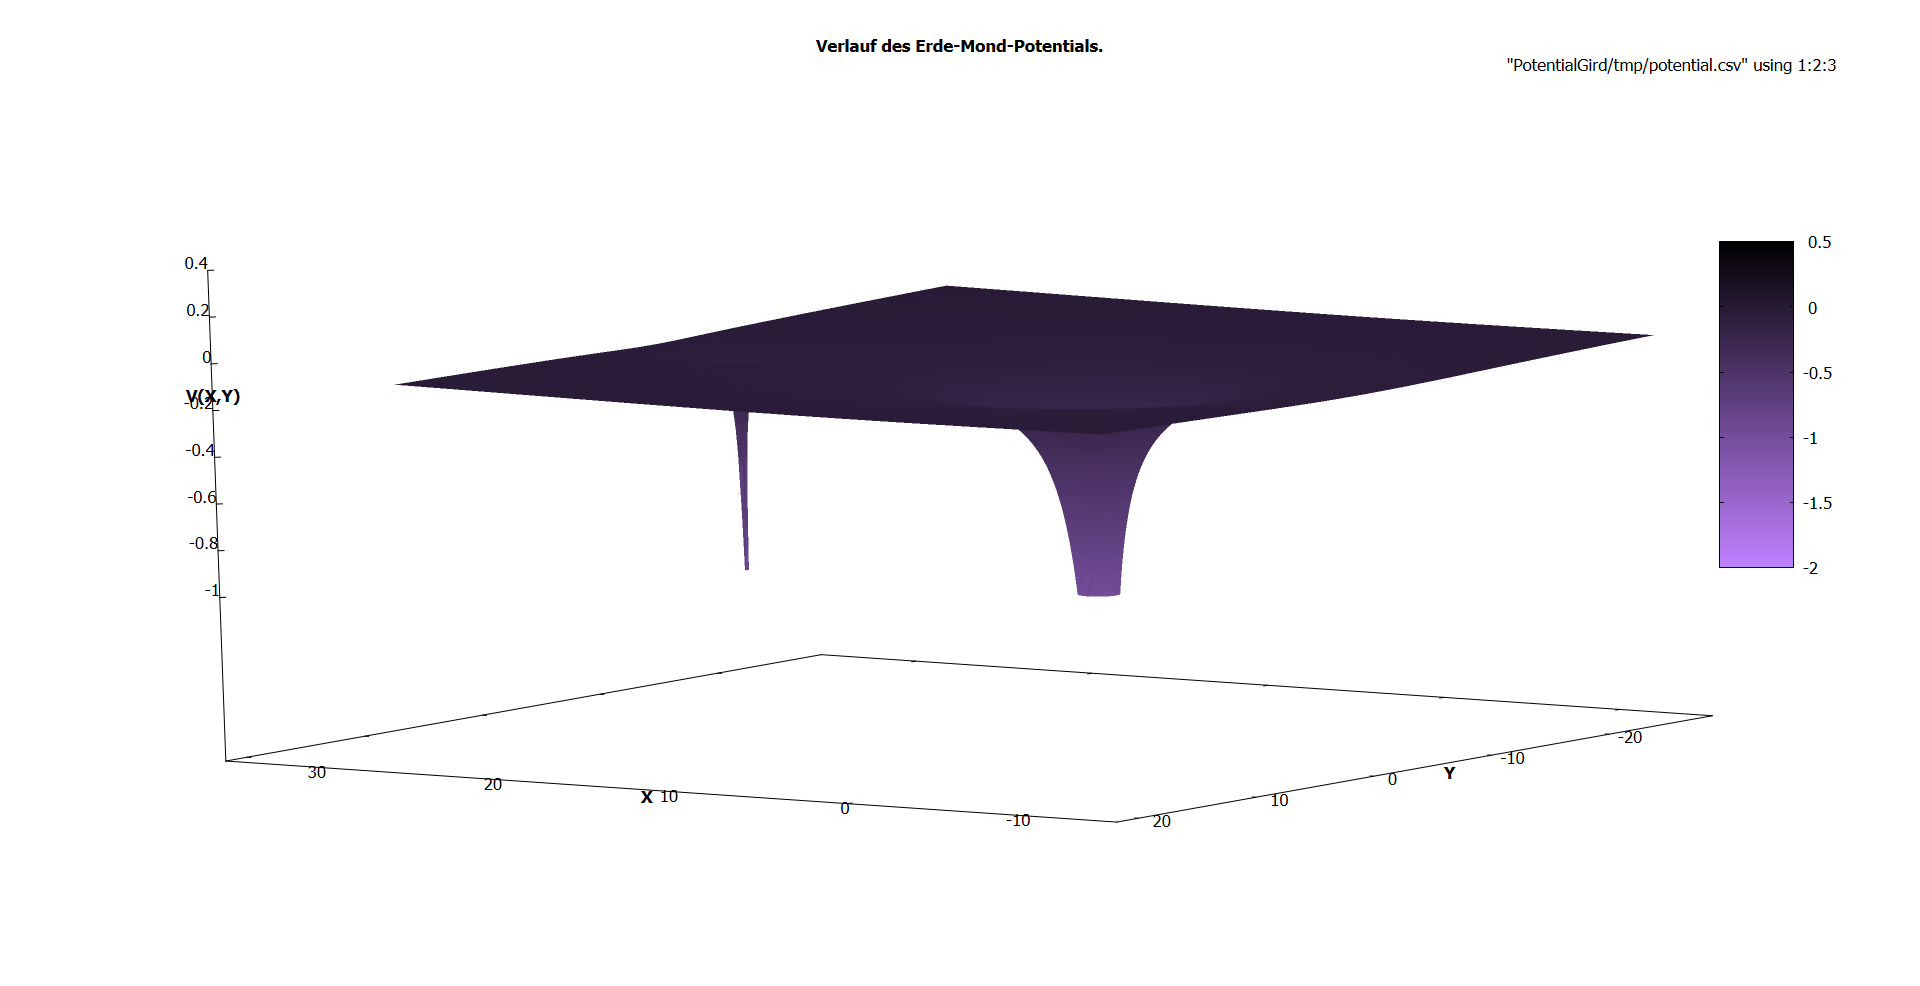
\includegraphics[width=0.8\textwidth]{../Ressource/PotentialVerlauf2.png}
        \caption{Potentialverlauf mit der kartesische Koordinate Darstellung}
        \label{fig:Potential}
    \end{figure}

    Wir haben uns aber während die Grundlagen Anteil für die kugelkoordinate Darstellung entschieden. Wir wählen eine Phase des Mondes
    $\Phi_M(t) = 0$ und ein Ellipsenparameter $a = 1$ Abstand Mond-Erde. Weiter ist der Azimutal-Winkel gleich 0 gestellt, sodass wir eine Projektions
    des Potentialverlaufes auf die $x$-$y$-Ebene erhalten.
    \begin{figure}[H]
        \centering
        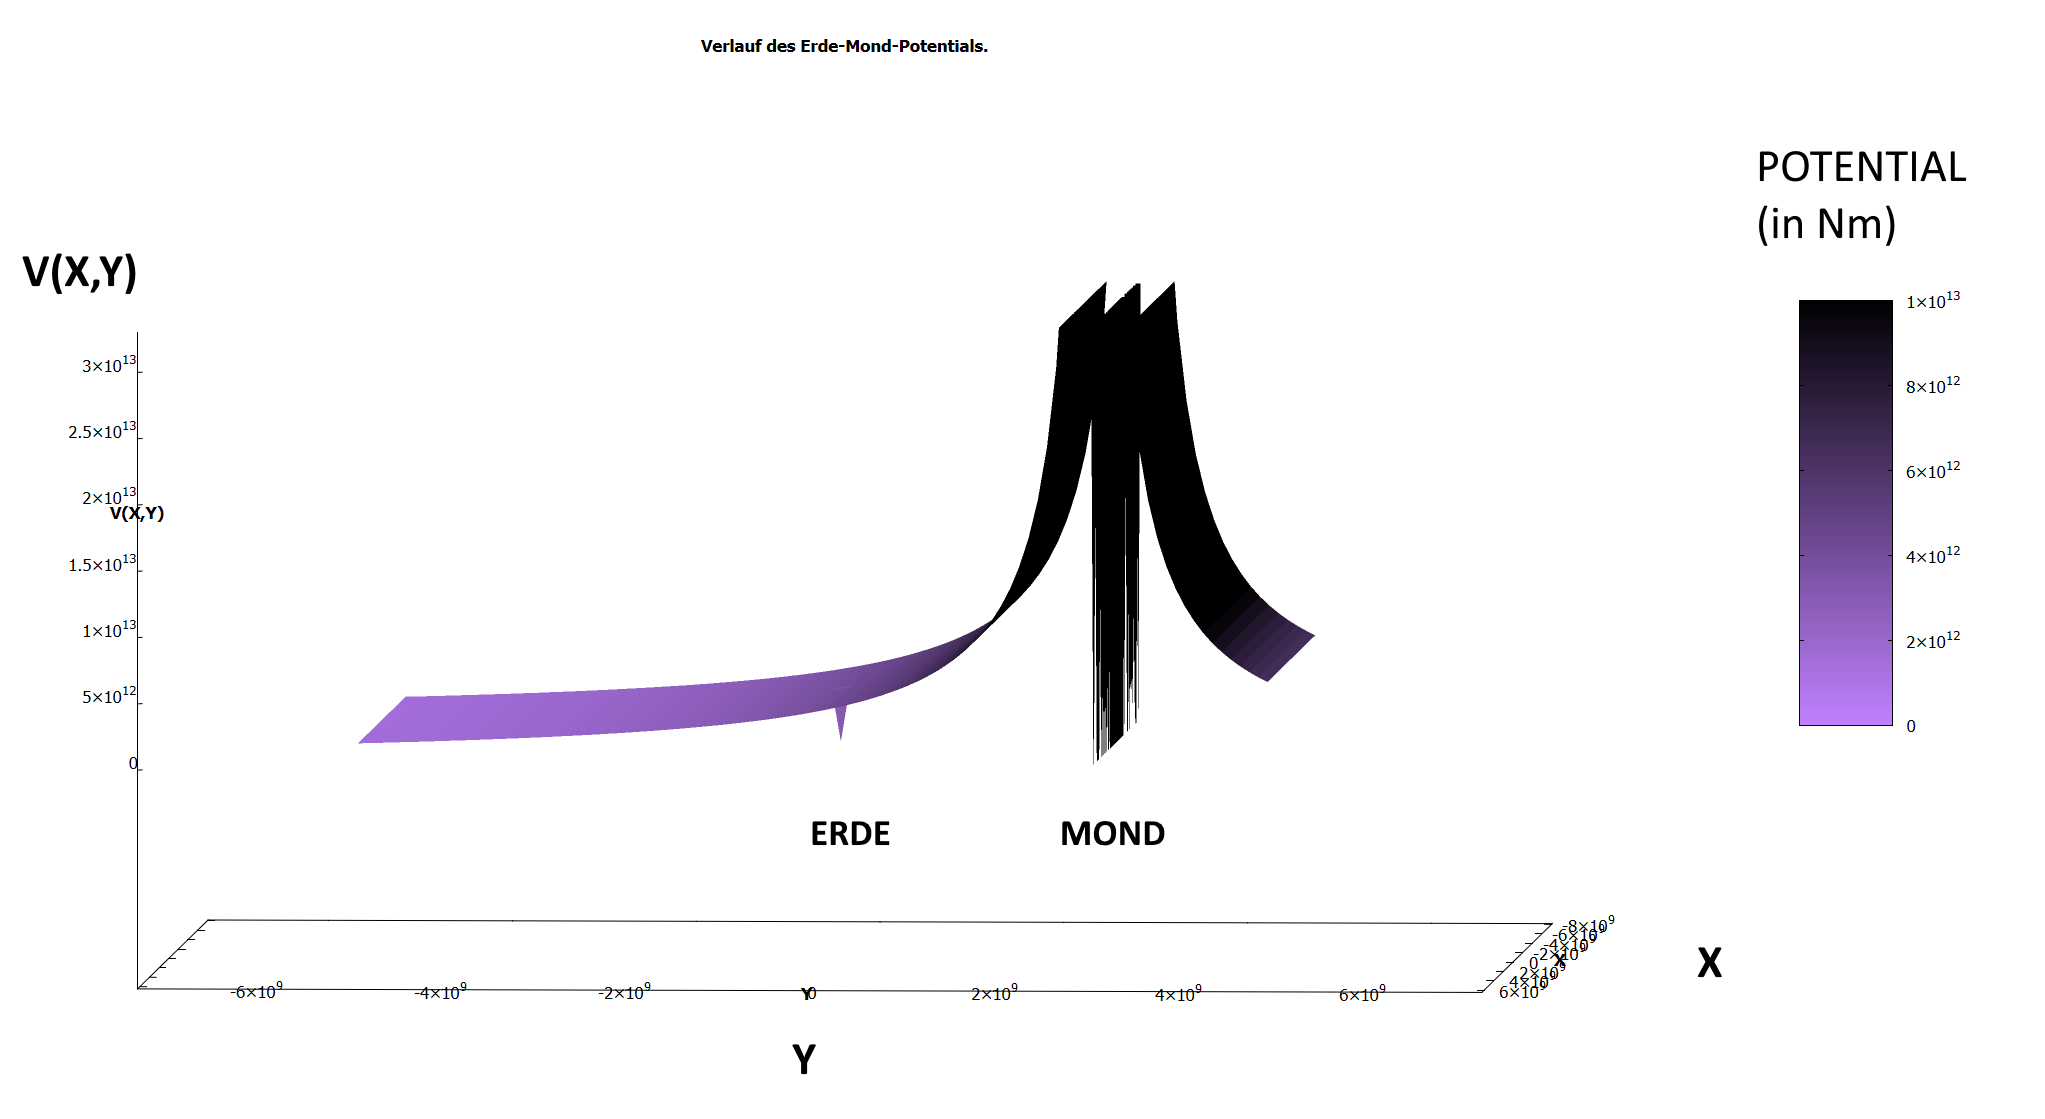
\includegraphics[width=0.8\textwidth]{../Ressource/PotentialVerlaufKugel.png}
        \caption{Potentialverlauf mit der kugelkoordinate Darstellung}
        \label{fig:PotentialKugel}
    \end{figure}
    Hier sieht man, dass wegen der arccos der Transformation ergibt es sich eine Asmyptote bei $\vec{y} = \vec{r}_mond$. Außerdem 
    funktioniert die $1/r$-Anteil für die Erde ganz gut.
    \paragraph{Schoss der Satelliten}$~$\\
    Zu jede Farbe gehört zwei Shosse. Hier haben wir einen Verfahren entwickelt, der den Anfangsimpuls in Richtung der Mond immer verbessert. Er basiert sich
    dafür auf die vorherige Anfangsimpuls der Simulation. Der Satelitt mit der kleinste Abstand zum Ziel wir als "besser" betrachtet.
    Wir schießen so 6 Paare von Satelitte. Wir haben das System in eine bewegende und fixe Mond betrachtet.\newline

    Für eine stehende Mond erhält man die folgende Schosse:
    \begin{figure}[H]
        \centering
        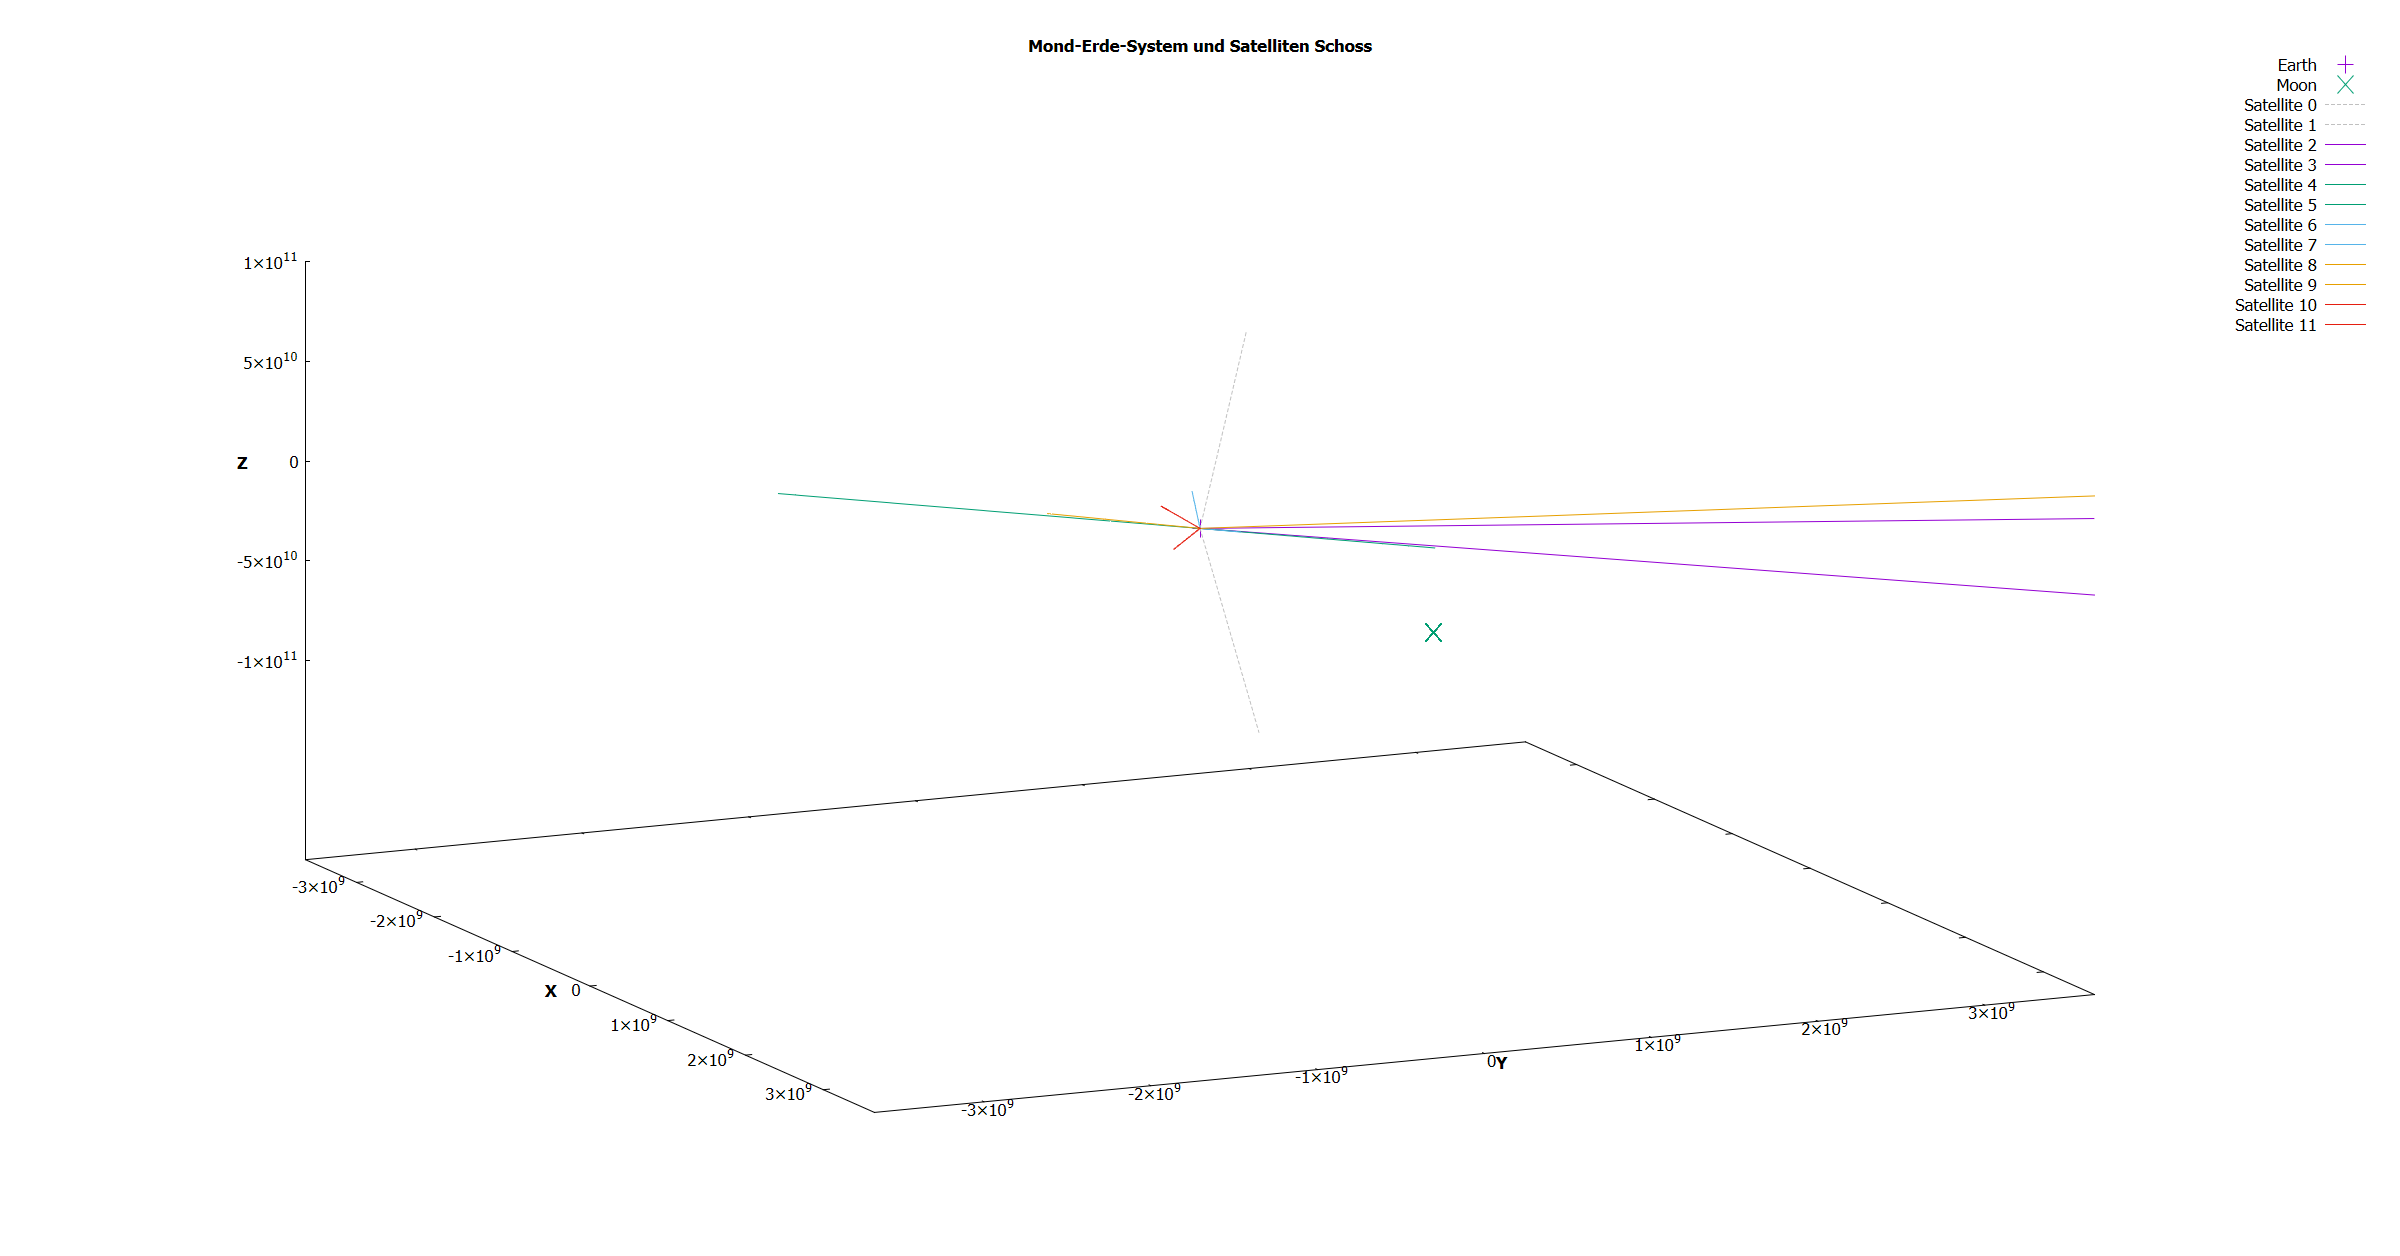
\includegraphics[width=1\textwidth]{../Ressource/Sat_fixeMond.png}
        \caption{Potentialverlauf}
        \label{fig:SatNoMon}
    \end{figure}
   Man sieht, dass die Trajektorien geradlinig sind. Die Sattelitten fliegen also in eine Richtung, und scheinen nicht von der Mond beeinflusst zu werden. 
   Die erste Schosse scheinen auf eine Ebene zu liegen. Die erste Hälfe fliegt nach rechts und der asimutale Winkel konvergiert gegen $\pi/2$. 
   Die Länge wird immer größer, d.h den Anfangsimpuls sleigt mit der Versuche. Ab der dritte Schoss fliegen die Satelliten nach links und den Winkel zur $x-y$ wird immer größer.Dafür ist die Länge kleiner, den Anfangsimpuls ist kleiner.  
    Für eine bewegende Mond erhält man die folgende Schosse:

    \begin{figure}[H]
        \centering
        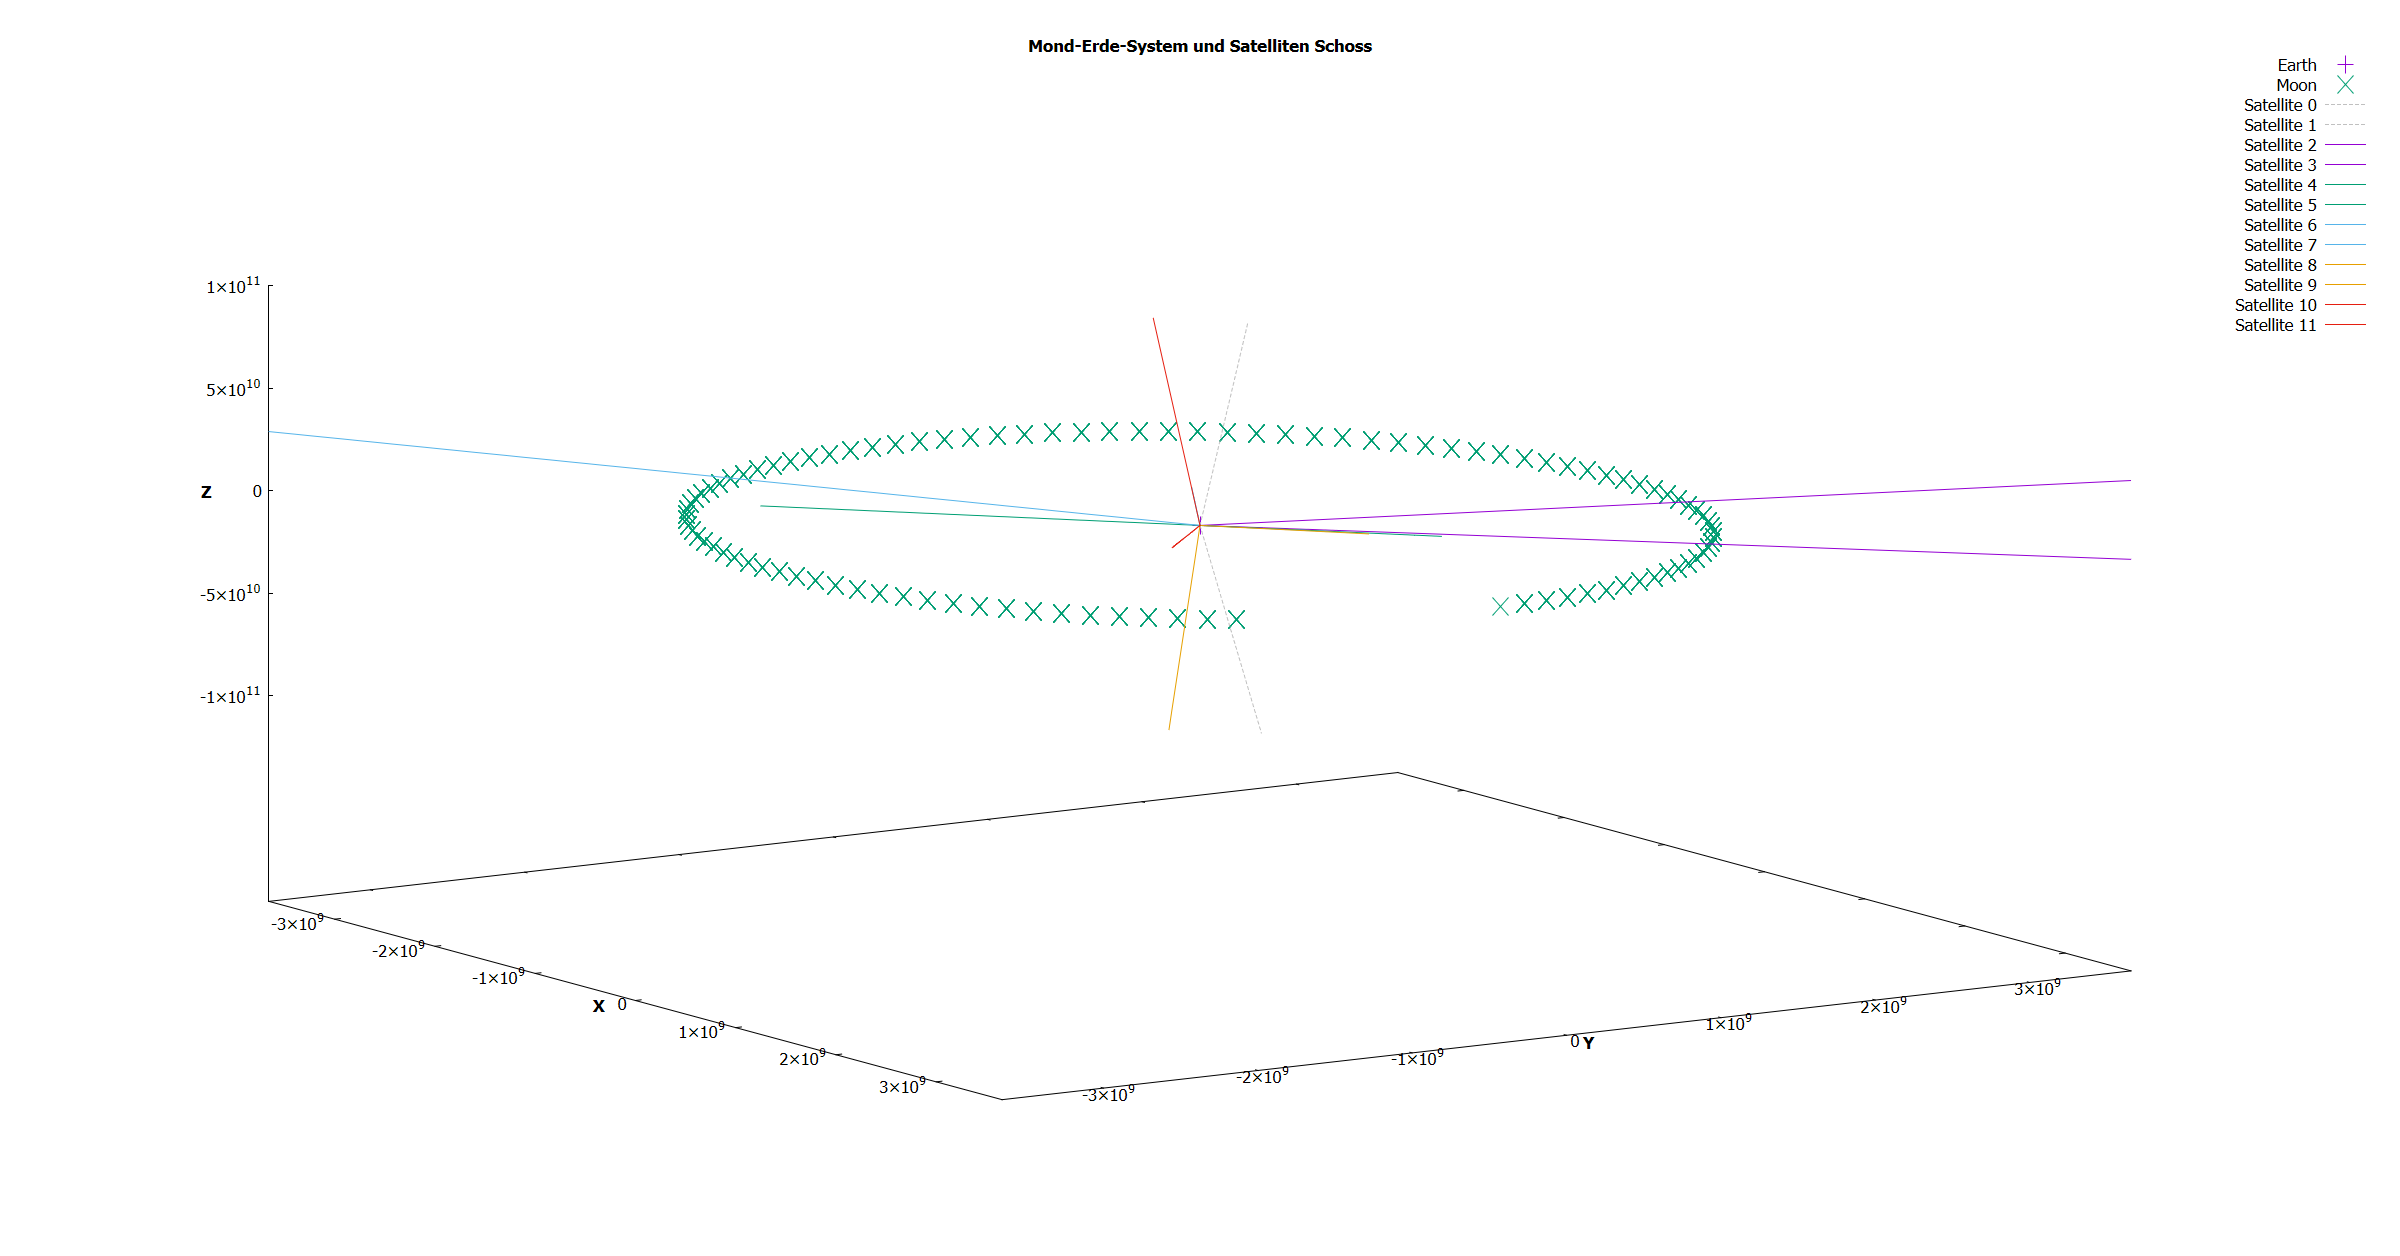
\includegraphics[width=1\textwidth]{../Ressource/Sat_moveMond.png}
        \caption{Potentialverlauf}
        \label{fig:SatWMon}
    \end{figure}
    Es ergibt sich dieselben Bemerkungen, obwohl den mond sich jetzt bewegt. Man sieht allerdings, dass die rote und gelbe Satelliten (i=5,6) in eine andere Richtung fliegen.\newline

    Wir hätten an dieser Stelle erwartet, dass die Trajektorie sich Richtung der Mond bewegt. Dies ist aber nicht der Fall. 
    Wir vermutten, dass eine Rechnung in der Vorbereitung schief gelaufen ist. Den Wahl von kugelkoordinate war vielleicht nicht so geschikt.
    Wir hätten das Problem in cartesiche kugelkoordinate lösen sollen. 
\end{document}